\documentclass[conference]{IEEEtran}
\IEEEoverridecommandlockouts
% The preceding line only needs to identify funding in the first footnote. If that is unnecessary, please comment on it.
\usepackage{cite}
\usepackage{amsmath,amssymb,amsfonts}
\usepackage{algorithmic}
\usepackage{graphicx}
\usepackage{textcomp}
\usepackage{listings}
\usepackage{xcolor}
\usepackage{bm}
\usepackage{hyperref}
\def\BibTeX{{\rm B\kern-.05em{\sc i\kern-.025em b}\kern-.08em
    T\kern-.1667em\lower.7ex\hbox{E}\kern-.125emX}}
\begin{document}

\title{Autonomous Design Report FS-AI\\[-0.3em]
{\Large Atlas Racing - Heriot Watt University Dubai}\\[-0.6em]
}

\author{\IEEEauthorblockN{Joseph Abdo, Moaiz Saeed, Aditya Shibu, Abdul Maajid Aga and Apsara Sivaprazad}
}

\maketitle

\begin{abstract}
This report outlines the development of an autonomous system by Atlas Racing ( Heriot-Watt University Dubai for the Formula Student UK Driverless (FS-AI) competition 2025. The system uses ROS 2 and integrates a 3d Lidar, stereo camera, GNSS, and IMU for perception and localisation. Google Cartographer was used for 3D SLAM, with an Extended Kalman Filter fusing GNSS and IMU data to produce accurate odometry. Cone detection and mapping were successfully implemented, enabling real-time localisation and navigation in a static environment. The system was deployed on the ADS-DV platform using the Jetson AGX Orin and achieved stable mapping and state estimation performance.
\end{abstract}

\section{System Architecture}
This section outlines the hardware and software architecture of the autonomous driving system deployed on the ADS-DV platform.  The entire software stack is developed using the ROS 2 (Robot Operating System 2) framework \cite{ros2humble}.

\begin{figure}[htbp]
\centerline{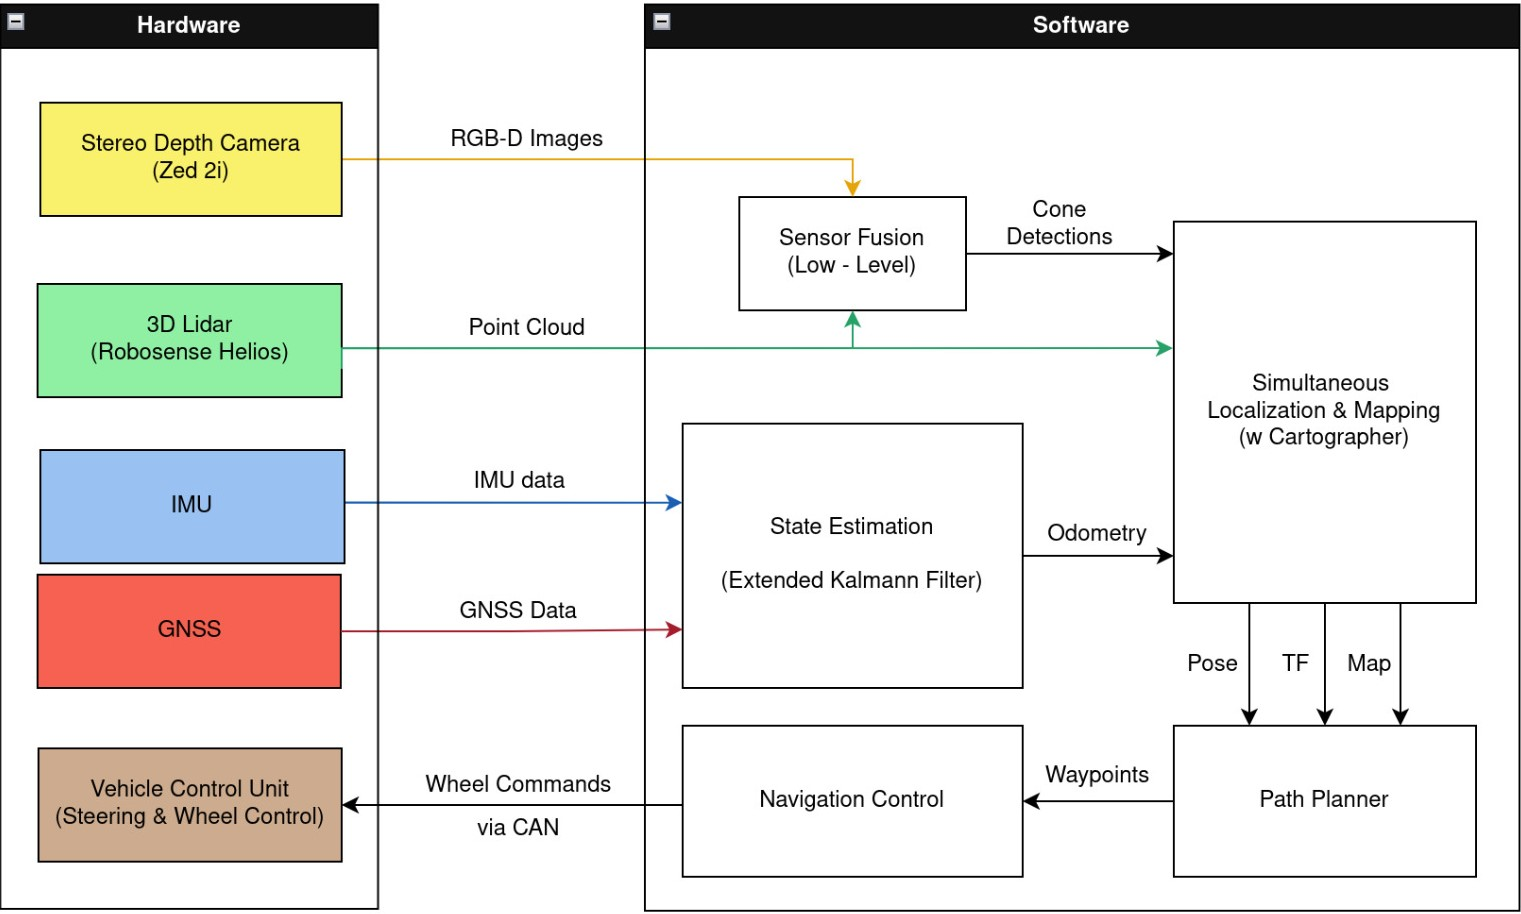
\includegraphics[scale=0.21]{images/System Arch.jpeg}}
\caption{High-level System Architecture}
\label{fig}
\end{figure}

\subsubsection{Sensors Onboard}
The perception stack includes a ZED 2i stereo depth camera and a RoboSense Helios 3D LiDAR sensor. The stereo camera provides synchronised RGB and depth images, while the Lidar sensor generates 3D point clouds, which allows for accurate spatial perception of the environment. For localisation, the system is also equipped with an IMU (Inertial Measurement Unit) and a GNSS (Global Navigation Satellite System) module \cite{stereolabs_zed2i} \cite{b3}. 

\subsubsection{Computing Module}
All sensor data is processed on the primary onboard computational unit, the NVIDIA Jetson Orin AGX module. It is selected for its high-performance GPU capabilities and low power consumption, making it suitable for real-time data fusion \cite{b4}. 

\subsubsection{Sensor Fusion}
Low-level fusion is performed on the inputs from the camera and LiDAR for cone detection. These detected features are essential for estimating the drivable space and forming a reliable map of the environment \cite{b14}.  

\subsubsection{SLAM}
The system uses an EKF (Extended Kalman Filter) to estimate odometry by fusing data from the IMU, GPS, and LiDAR sensors\cite{b7}. The odometry and the cone detections are provided to the Cartographer SLAM (Simultaneous localisation and mapping) framework to perform real-time simultaneous localisation and mapping. The output of Cartographer is a continuously updated global map that reflects the vehicle’s environment and position within it \cite{b5} \cite{b6}.

The generated map is fed to the path planning module, which computes a sequence of waypoints to the current navigation objectives. This module sets environmental constraints and vehicle dynamics to ensure the generated trajectory is fail-safe. 

\subsubsection{Navigation Control}
The final stage of the pipeline involves the navigation control module, which uses the computed waypoints to derive vehicle kinematics. It then generates wheel commands to appropriately steer, throttle, or brake the vehicle. These commands are transmitted to the ADS-DV (Autonomous Driving Systems-Dedicated Vehicle) platform via a CAN (Controller Area Network) bus interface, completing the control loop.

\section{Perception}
This section details the implementation of the vehicle's perception system, explaining how it interprets its environment using both LiDAR (laser-based) and vision-based technologies.

\subsection{LiDAR (laser-based)}\label{AA}
The RoboSense Helios series Lidar with a 16-beam configuration was selected, offering a balanced trade-off between angular resolution, detection range, update rate, and cost-effectiveness. Filtering and clustering techniques enhance data reliability and remove irrelevant or noisy points that could interfere with path planning. The code detection pipeline using LiDAR follows a multistage approach, as outlined below:
\subsubsection{Raw Data Acquisition}
Data is captured as points in 3D space and transformed to the vehicle's reference frame using sensor\_transform matrices. The system implements a thread-based processing with Mut-Ex (Mutually Exclusive) locks to ensure thread safety while maintaining real-time performance.
\subsubsection{Point Cloud Filtering and Accumulation}
Employing several filtering strategies:
\begin{itemize}
    \item Distance-based filtering:
    \[
    \mathit{close\_points\_mask} = \left( d < 50.0 \right)
    \]
    Where \textbf{‘d’} is the distance to each point, this step filters out all points beyond 50 meters, allowing the system to focus on relevant track sections.

    \item Height-based filtering:
    \[
    \mathit{near\_ground\_mask} = \left( z < h_{\text{ground}} + 0.5 \right) \land \left( z > h_{\text{ground}} \right)
    \]
    where \textbf{‘z’} is the z-coordinate of the LiDAR points, and \textbf{‘$\bm{h_{\text{ground}}}$’} denotes the estimated ground height.

    \item Point accumulation: Points from multiple frames are appended to improve cone detection density, especially in sparse or occluded regions.
\end{itemize}

\subsubsection{Cone Identification}

The cone identification uses DBSCAN (Density-Based Spatial Clustering of Applications with Noise) clustering with the parameters eps=0.5 and min\_samples=5; finding this to be the sweet spot, which gave a good balance between noise reduction and the ability to detect distinct clusters in the data points. The team proceeded with DBSCAN over alternatives such as OPTICS (Ordering Points To Identify the Clustering Structure) because DBSCAN offers better computational efficiency at O(n log n) vs. O(n\textsuperscript{2}) \cite{b8}, which is critical for real-time performance. Although OPTICS provides more flexibility, since such granularity was unnecessary in this context, where cones are relatively uniform in size and spacing, DBSCAN effectively filters out noise while reliably clustering actual cone detections \cite{b9}.
\vspace{0.2em}
\subsubsection{Cone Validation}
Cone detection is done through size validation, ensuring that each cluster matches the expected physical dimensions of a cone. This is followed by confidence scoring, which evaluates point density and other cluster characteristics. Additionally, multi-frame tracking is implemented to reduce false positives and enhance detection stability over time.

\subsection{Image and Object Detection (vision-based)}
The object detection system is designed to accurately identify and classify the track cones in real-time while providing precise spatial information for navigation. After several approaches, YOLOv8 was selected as the primary detection model.

\subsubsection{Model Development and Training}
Three cone datasets from Kaggle were created to form a unified training dataset with standardised labelling conventions. The classification scheme used numeric labels (0=orange, 1=yellow, 2=blue, 3=large orange, and 4=unknown) to ensure consistent identification across various racing environments. The training process involved a train-test split of 80\% (10,003 images) 20\% (10\% validation, and 10\% testing, 1,250 images each) along with a training configuration with 100 epochs, 32 batches, and 25 early stopping patience \cite{b10}\cite{b11}\cite{b12}. 

\begin{figure}[htbp]
\centerline{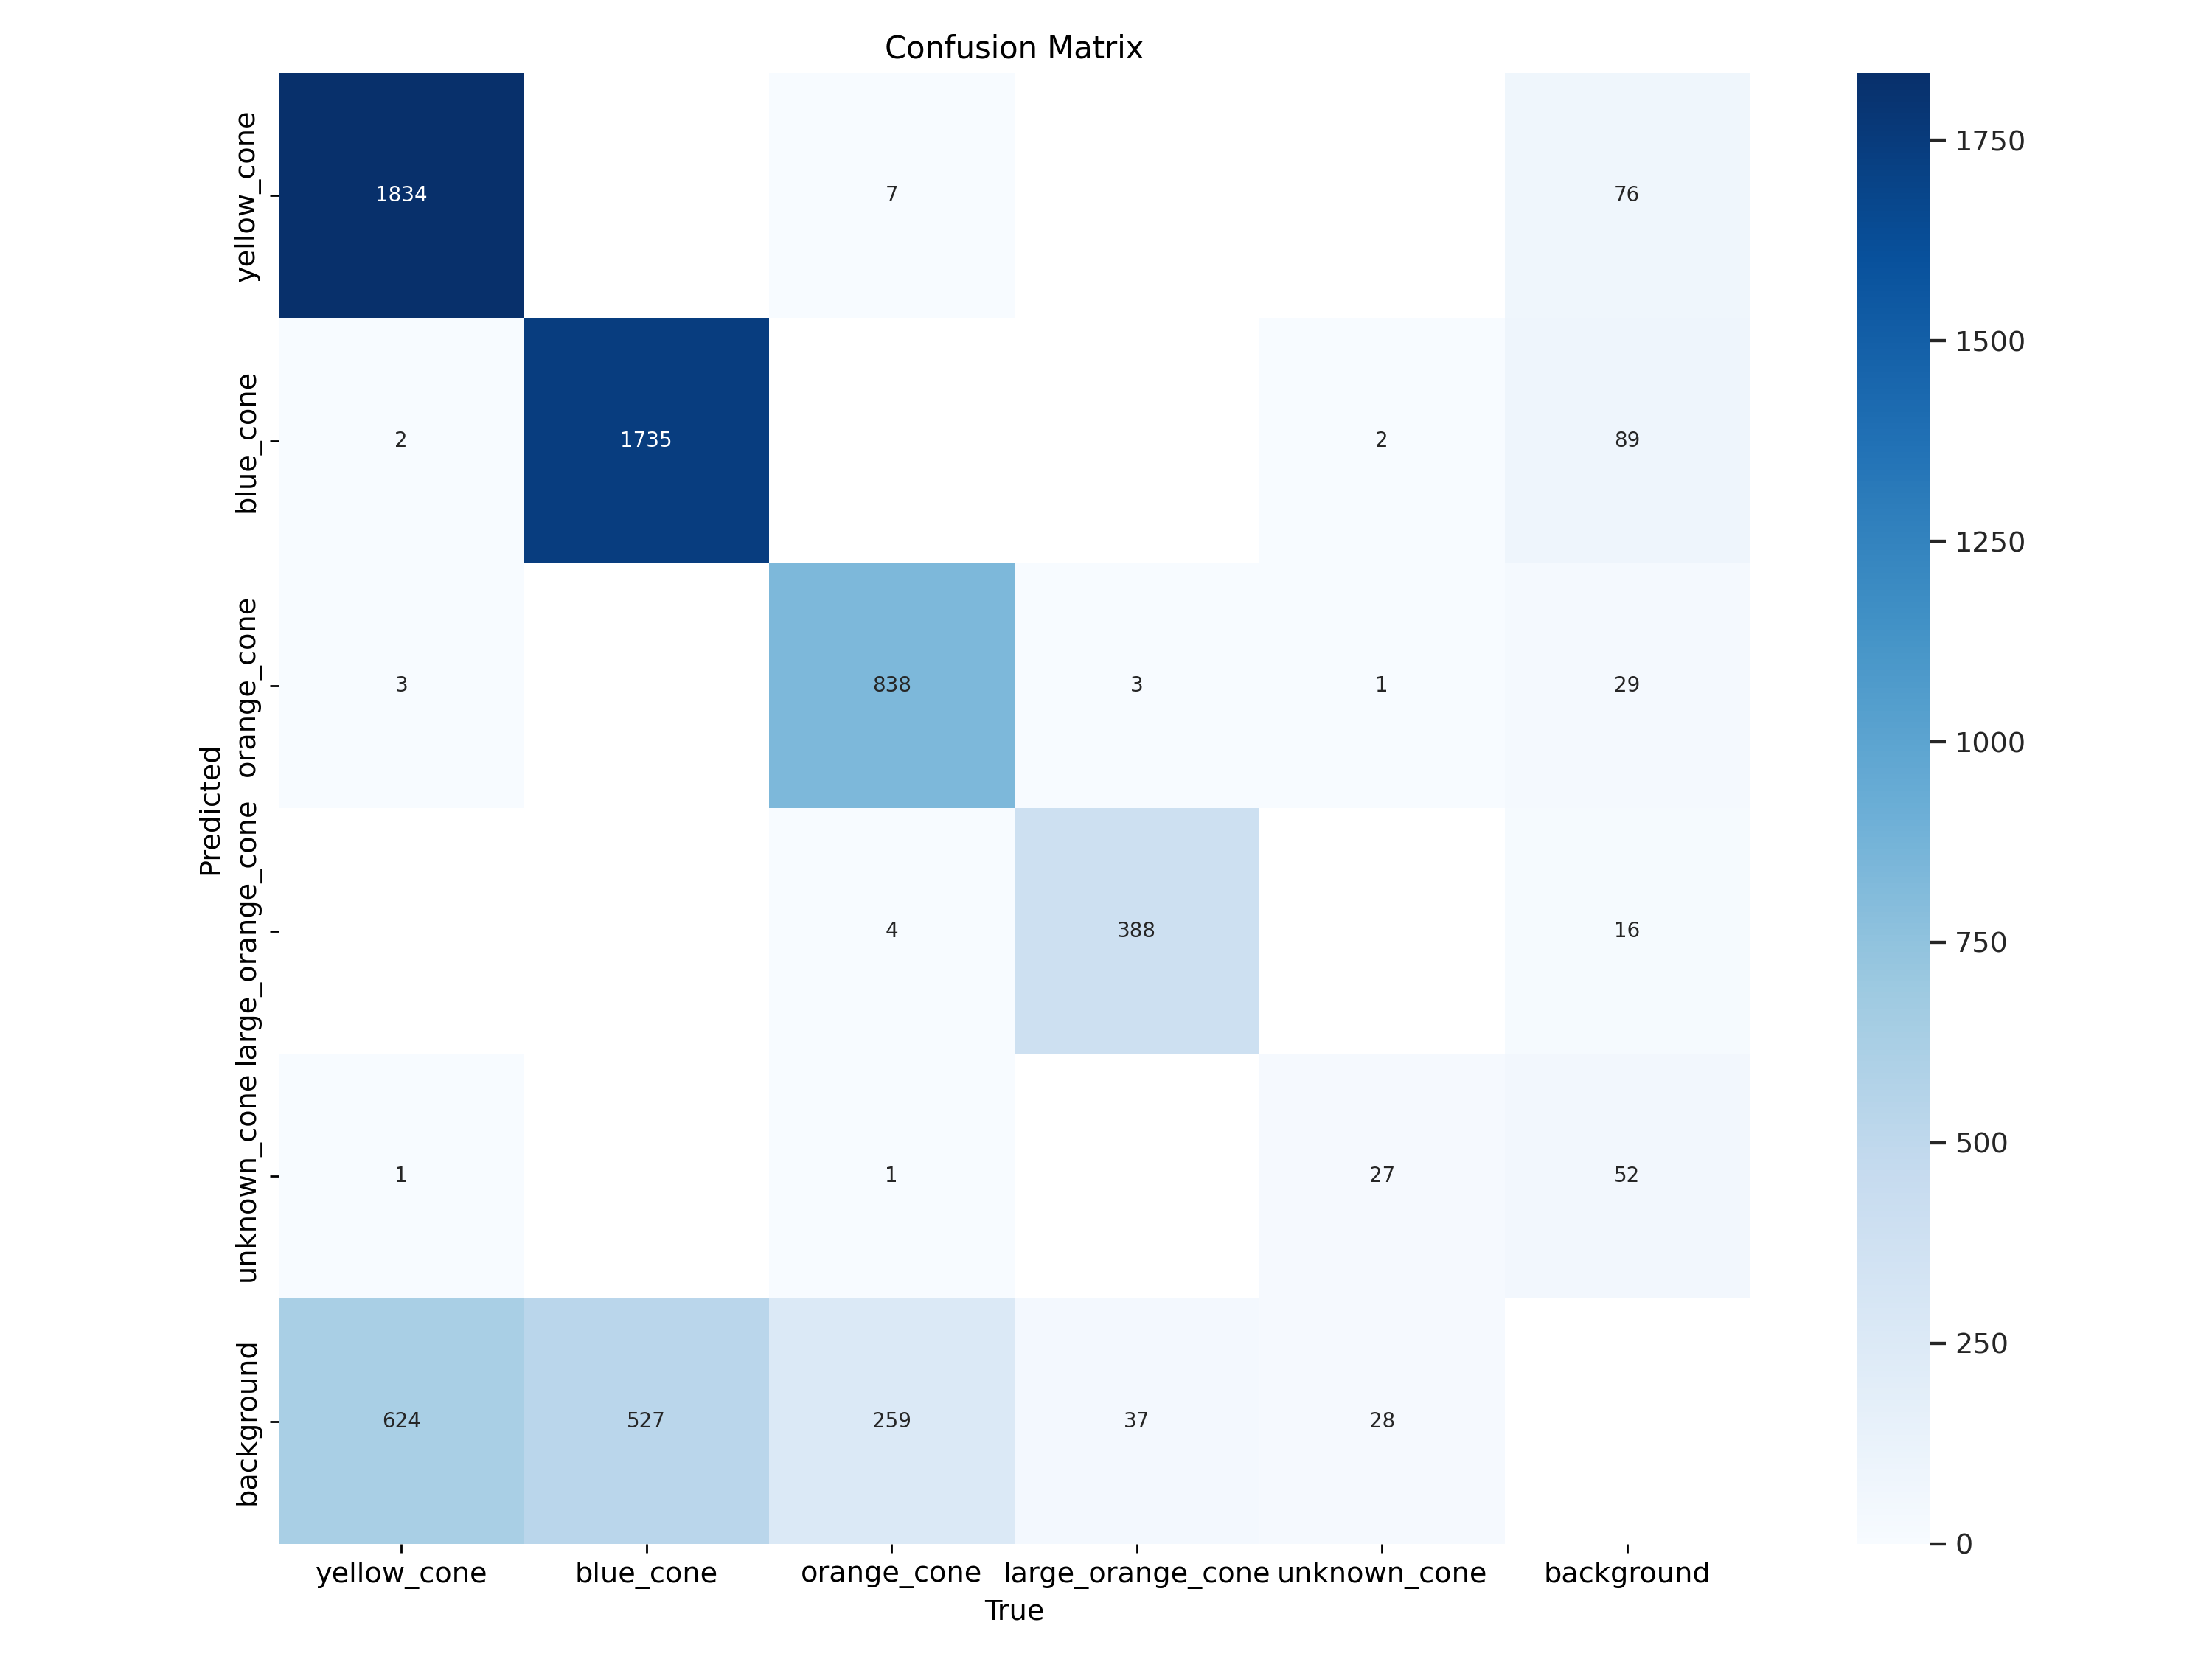
\includegraphics[scale=0.3]{images/confusion_matrix.png}}
\caption{Confusion Matrix of the trained YOLO Model}
\label{fig}
\end{figure}

\textbf{Testing Result:} The model accuracy is shown in Figure 1, with appropriate results for yellow and blue cones (highest actual favourable rates). The confusion matrices revealed that most misclassifications occurred between visually similar cone types.

\subsubsection{YOLOv8 vs. HOG Performance Analysis}
On comparing YOLO (You Only Look Once) and HOG (Histogram of Oriented Gradients) with SVMs (Support Vector Machines), referencing Kaplan and Şaykol's research. Although HOG with SVM achieved an 86.7\% success rate when trained on 80\% of the dataset, YOLO demonstrated superior reliability and accuracy in racing environments with significantly fewer false positives (5 vs. 84 for HOG), Higher actual positive detection rate (218 vs. 154 for SVM) and a better overall performance in dynamic racing environments \cite{b13}.

\subsubsection{Performance metrics and Evaluation}
Model evaluation demonstrated the relationship between confidence thresholds and detection accuracy. The F1 score peaked between confidence thresholds of 0.1 and 0.6. Precision remained high across most confidence levels for all cone classes. Recall started high at low confidence thresholds, stabilised between 0.6 and 0.4, and then dropped at higher thresholds.

\begin{figure}[htbp]
\centerline{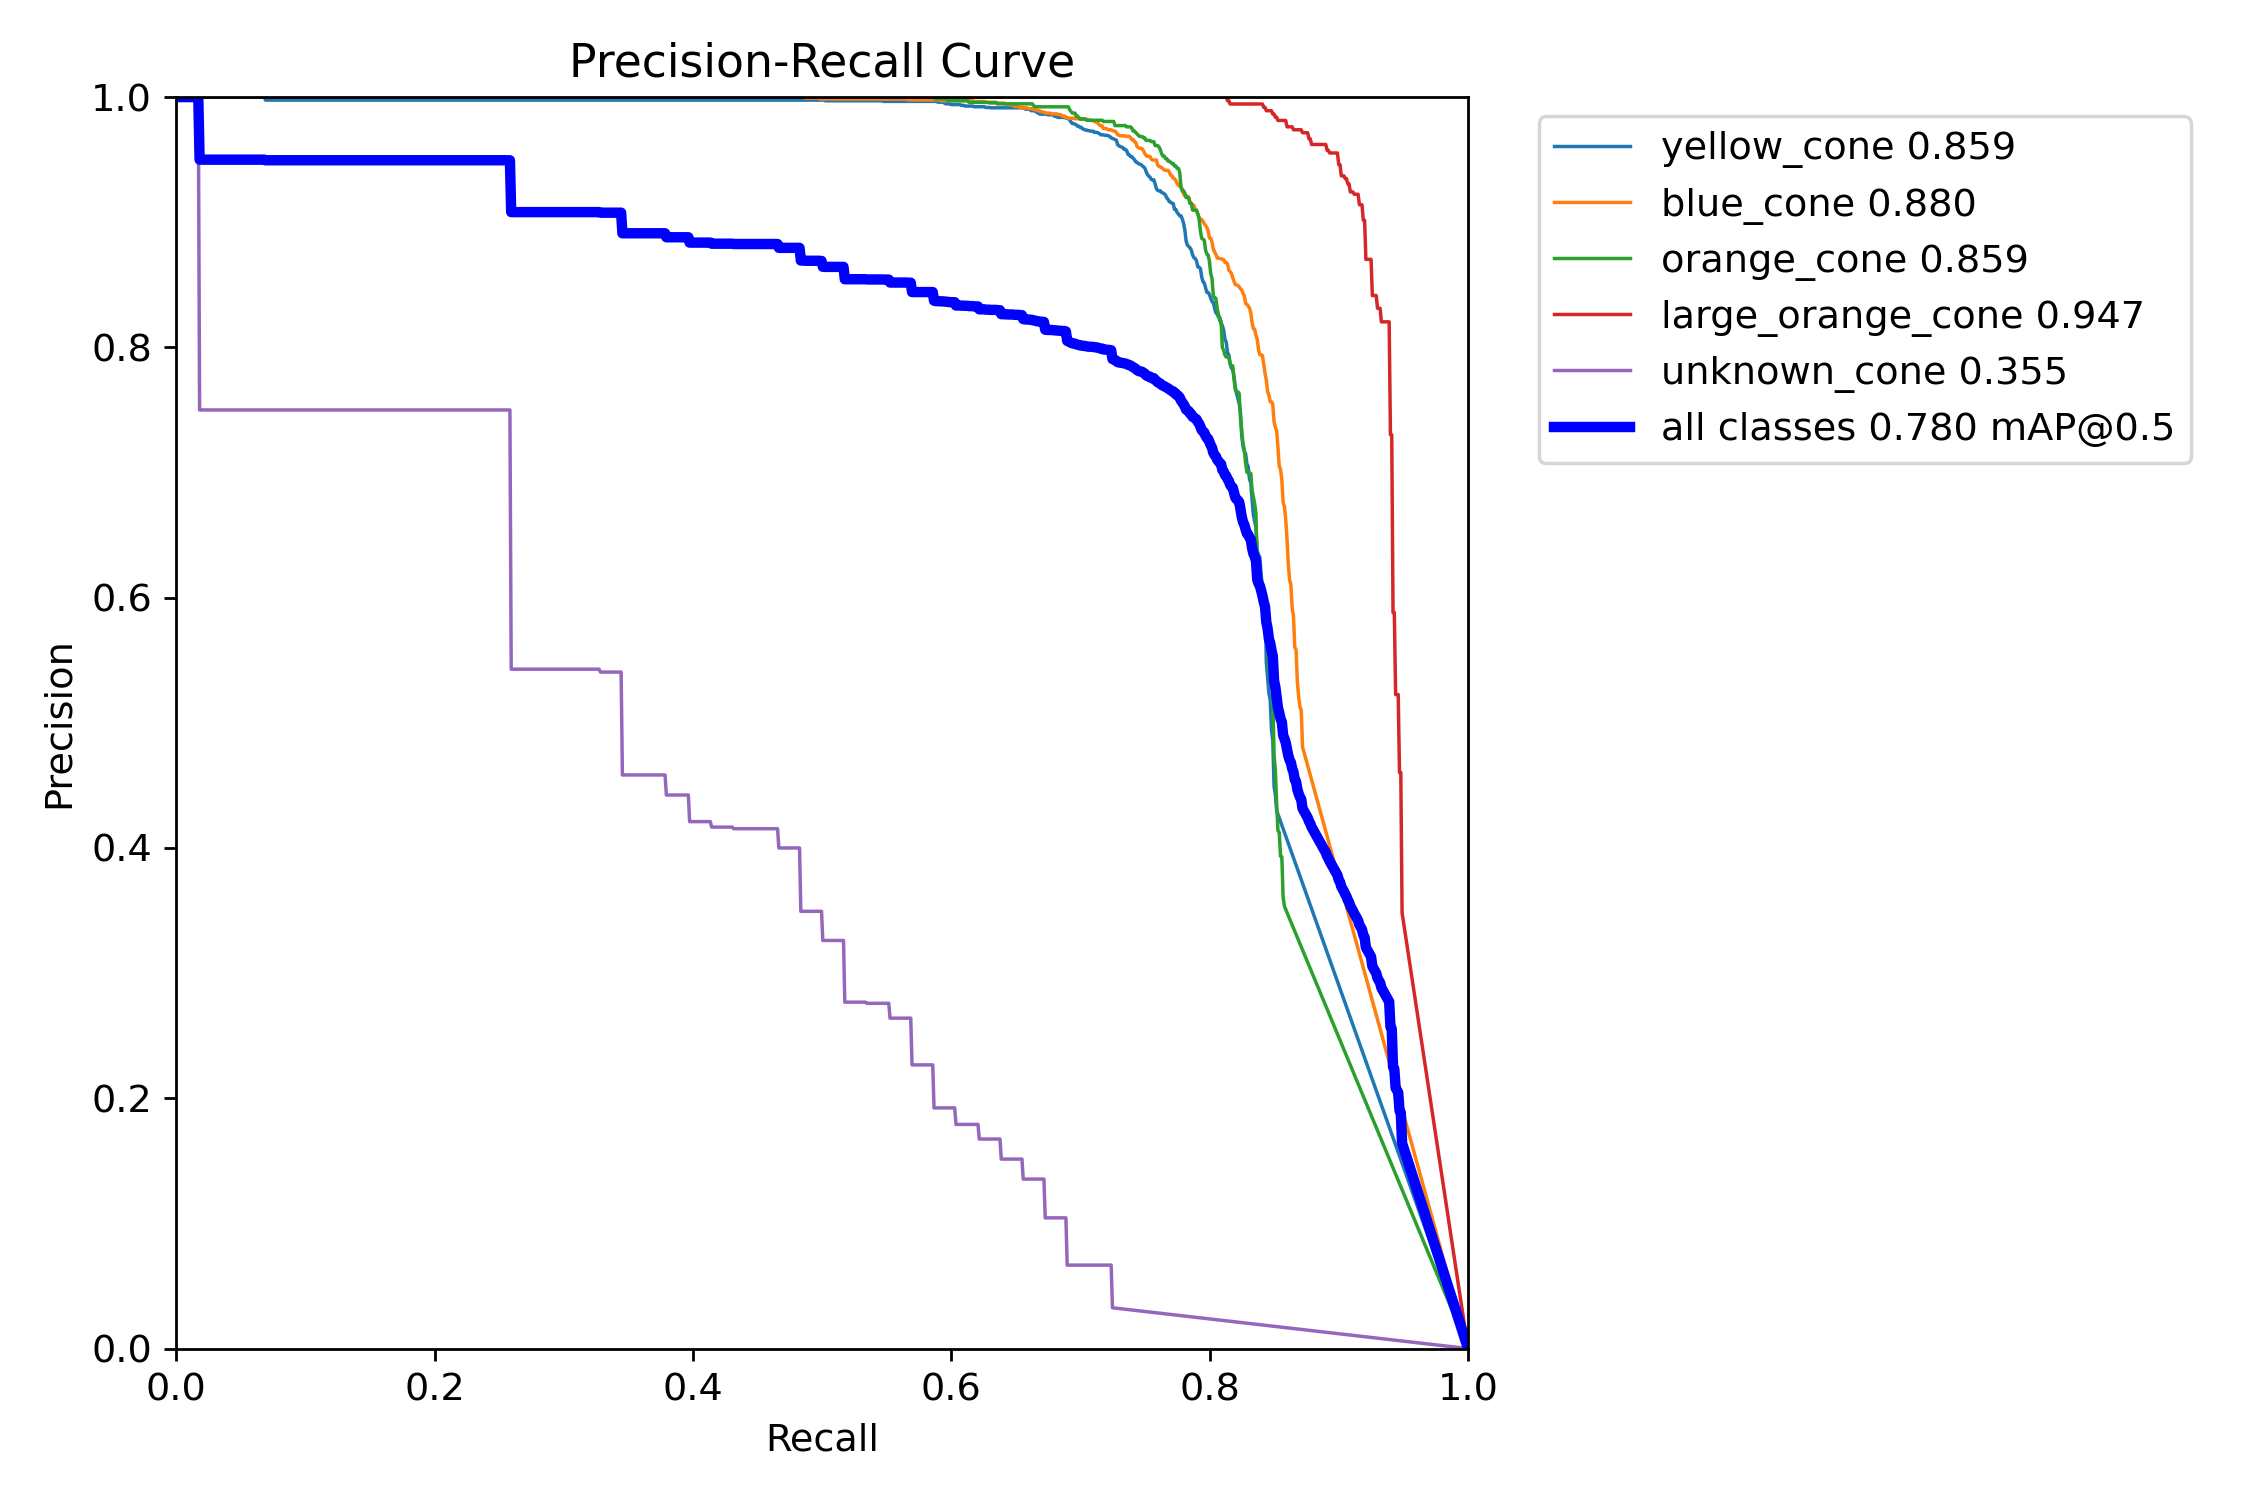
\includegraphics[scale=0.4]{images/PR_curve.png}}
\caption{Precision-recall curve}
\label{fig}
\end{figure}

\begin{figure}[htbp]
\centerline{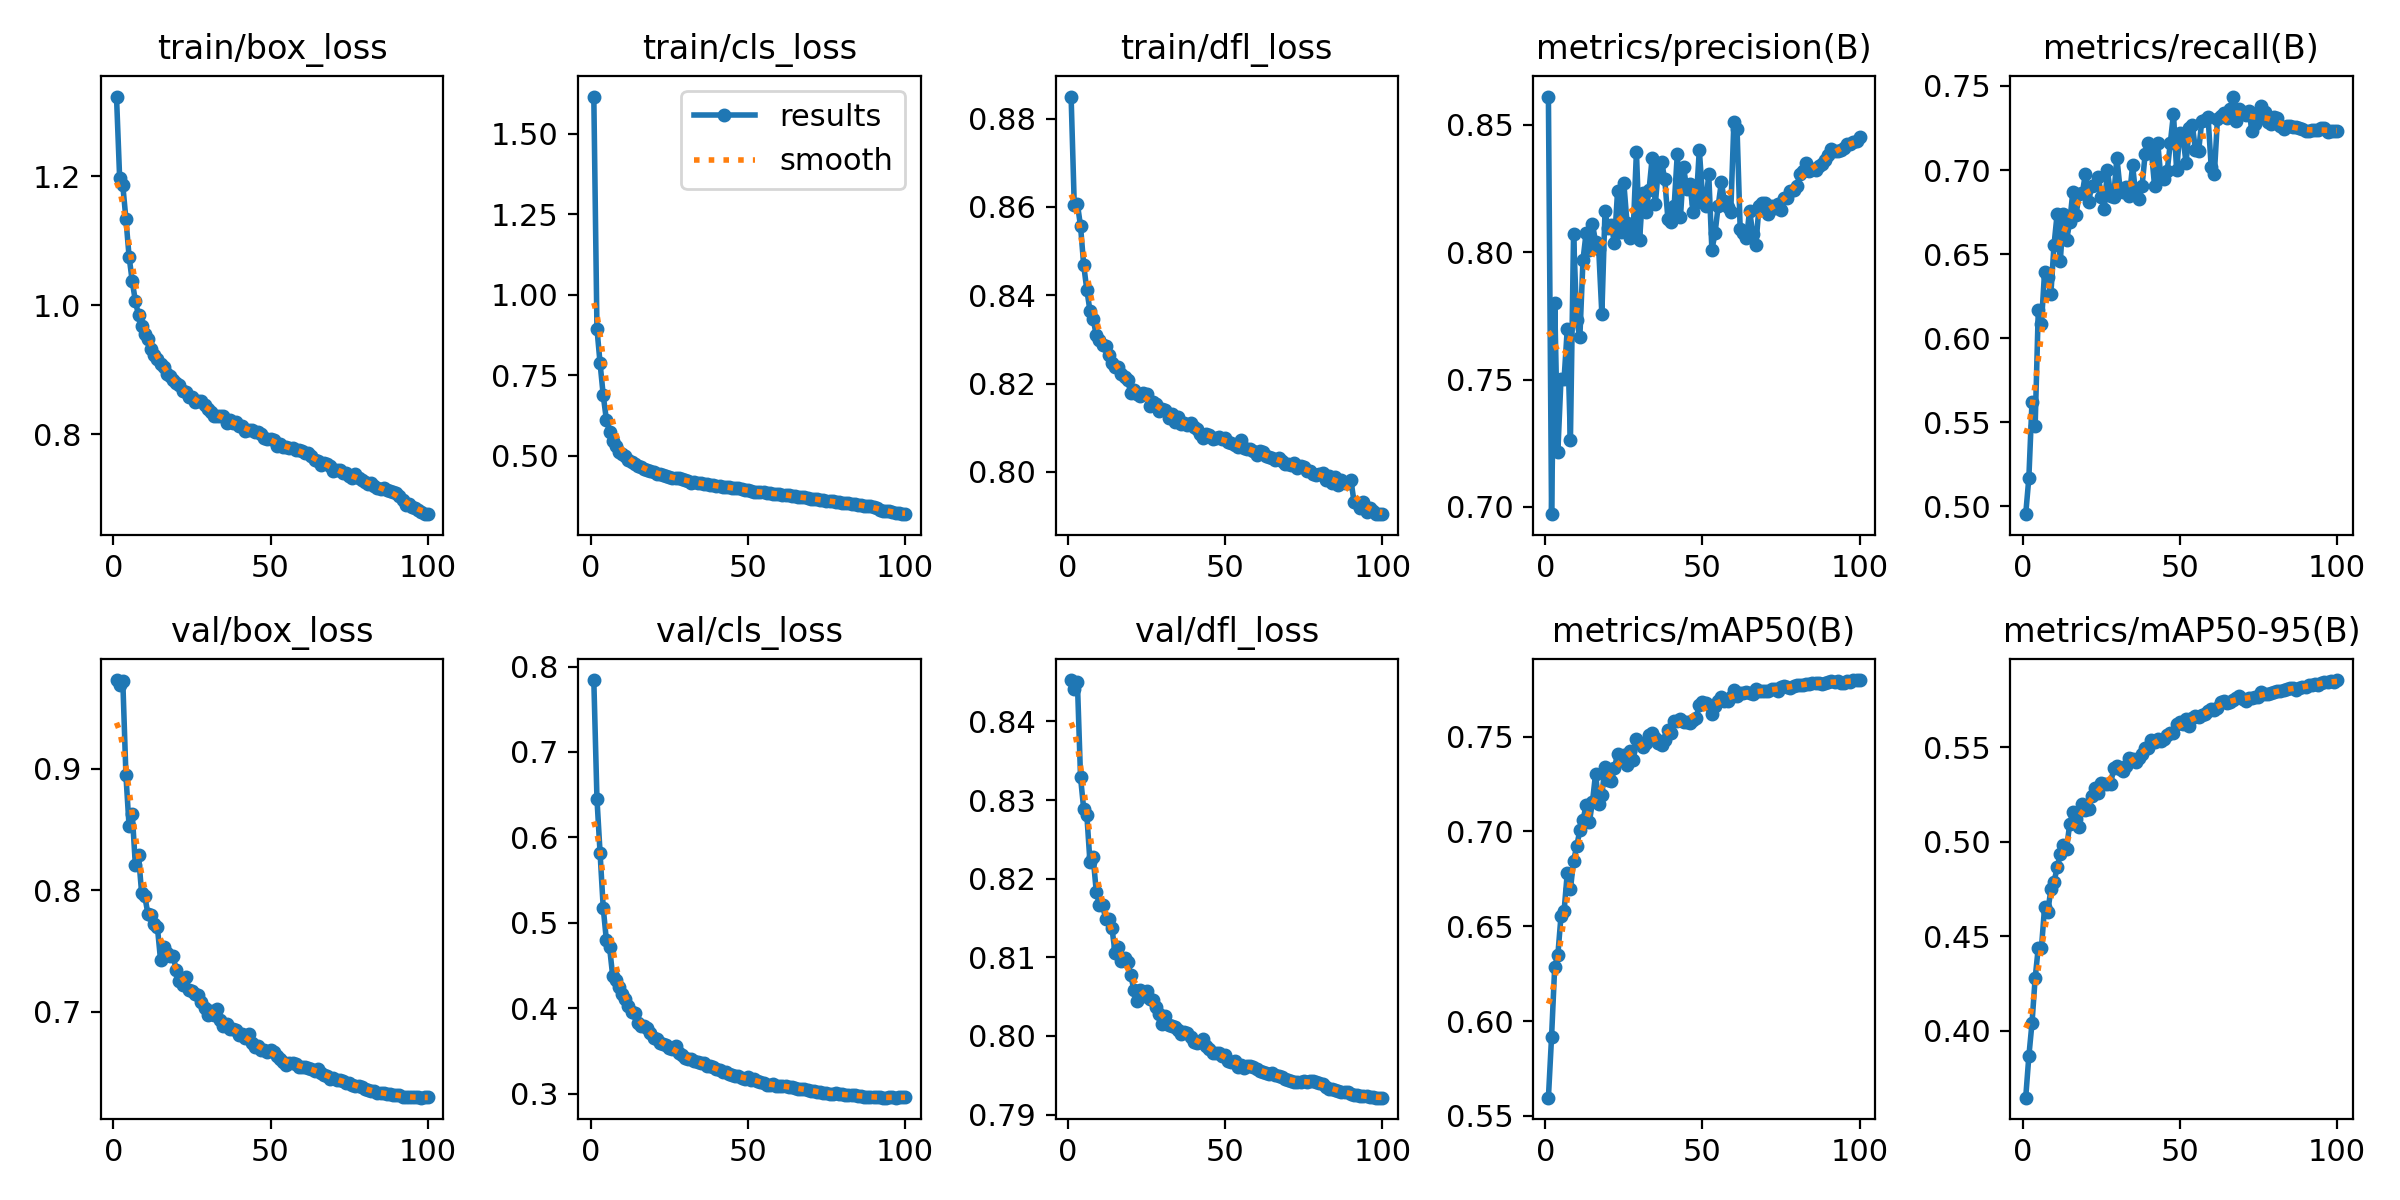
\includegraphics[scale=0.3]{images/results.png}}
\caption{Training metrics graph}
\label{fig}
\end{figure}

The precision-recall curve (Figure 2) illustrates the trade-off between detection accuracy and coverage. The training metrics (Figure 3) showed consistent improvement across epochs for bounding box loss, classification loss, and mean average precision (mAP), confirming stable training without significant overfitting.

\subsection{Depth Camera (vision-based)}
The system uses the ZED 2i stereo camera as a secondary perception pipeline to enhance system reliability through sensor fusion and provide critical colour classification capabilities that complement the Lidar system. The ZED 2i was explicitly selected for its built-in stereo capabilities that provide accurate depth measurements up to 20m, critical for cone detection requirements. The camera subsystem consists of two primary components.

\subsubsection{Advanced Depth Estimation}
A key innovation in the system is a multi-faceted depth estimation approach that combines several techniques: direct depth sampling from the stereo camera's depth map, temporal smoothing using a sliding window of recent detections, position-based depth estimation, and box–size–normalised depth correction. The final depth is computed as:
\[
\textit{final\_depth} = 0.5 \cdot \textit{smoothed\_depth} + 0.5 \cdot \textit{position\_depth}
\]
This provides more reliable depth estimates than any single method alone. This approach is particularly effective at handling the rapidly changing distances encountered in racing scenarios.

\subsubsection{Track Boundary Visualization}
The system automatically identifies and visualises track boundaries by first classifying detected cones based on colour (yellow, blue, and orange). The cones are sorted by depth to determine their sequence along the track. To visually represent the track edges, lines are drawn between consecutive cones of the same colour. This process provides precise visual feedback that supports real-time path planning and offline validation, helping to ensure accurate and reliable vehicle navigation.

\vspace{0.4em}
Through extensive testing, it was concluded that a camera-based perception system achieved detection ranges of 1-20m with centimetre-level accuracy after calibration. The integration with the Lidar system through sensor fusion not only improved overall detection reliability but also colour-based cone detection, which simplified the path planning algorithm.

\subsection{Laser-vision Fusion}\vspace{-0.4em}
The system employs a fusion technique to combine LiDAR data with camera detections, leveraging the strengths of both perception systems to create a more robust and reliable cone detection system.

\subsubsection{Low-level Fusion Approach}
While many autonomous racing solutions employ mid-level fusion due to its lower computational complexity, our system implements low-level fusion to achieve peak performance and racing speeds on track. This approach processes raw data from both sensors jointly before making detection decisions, providing key advantages such as enhanced detection accuracy through complementary sensor information, Improved reliability across a wide range of weather conditions, More precise spatial localisation by combining depth information from multiple sources, and reduced false positives through cross-validation between sensors \cite{b14}.

Although the low-level fusion approach is computationally more demanding, it yields superior detection quality. It is critical for the high-speed racing environment, where precise cone positioning is essential for optimal path planning.

\subsubsection{Sensor Alignment and Calibration}
The fusion pipeline begins with sensor alignment using rigid transformation matrices between the LiDAR and camera reference frames, depth correction factors to address systematic sensor biases, and point cloud projection into the camera's image plane for correlation. These calibration steps ensure data from both sensors is registered in a standard coordinate frame before fusion.

\subsubsection{Data Association and Fusion Algorithm}
The core of the fusion system is a matching algorithm that associates LiDAR-detected cone clusters with camera-detected bounding boxes using the following steps:
\begin{itemize}
\item Projection Step: Lidar points are transformed to the camera frame and projected onto the image plane using the camera's intrinsic parameters
\item Association: Each 3D point is matched with its corresponding 2D detection using a weighted distance metric that considers both spatial proximity and confidence scores
\item Confidence Fusion: For matched detections, a confidence-weighted averaging is performed using the equation:
\begin{equation}
P_{\text{fused}} = \frac{P_{\text{camera}} \cdot w_{\text{camera}} + P_{\text{LiDAR}} \cdot w_{\text{LiDAR}}}{w_{\text{camera}} + w_{\text{LiDAR}}}
\end{equation}
Where \textbf{‘P'} stands for the position and \textbf{‘w'} stands for the weight/confidence \cite{b15}.
\item Classification Transfer: Colour information from the camera detections is transferred to the corresponding LiDAR points
\item Unmatched Point Handling: Points detected by only one sensor are preserved but assigned a reduced confidence score to maintain the continuity of detection
\end{itemize}

\subsubsection{Adaptive Confidence Weighting}
The system employs dynamic confidence weighting that adjusts based on sensor reliability under different conditions. For example, when Camera detection confidence is weighted higher in good lighting conditions, LiDAR measurements are prioritised in low-light environments or at longer distances. Distance-dependent weighting gives preference to the camera for colour classification and LiDAR for precise positioning, and Historical detection consistency is factored into confidence calculations.

This adaptive approach ensures optimal fusion performance across the diverse conditions encountered during the competition.

\subsubsection{Performance Improvements}
Although the system initially employed a mid-level fusion approach, the decision was made to transition to a low-level fusion due to mid-level fusion causing lower vehicle speeds. Specifically, the mid-level fusion method introduced delays, requiring each sensor to detect and process data independently before fusion. Low-level fusion integrates raw sensor data prior to processing, significantly reducing latency. This shift resulted in several key improvements, including an extended detection range exceeding 20m, cone colour classification accuracy above 98\%, reduced overall detection latency, and enhanced tracking continuity during temporary sensor occlusions.

These improvements directly translate to higher racing speeds and more accurate path planning, giving the vehicle a competitive edge.

\section{SLAM}
State Estimation is used to generate an accurate mapping of the environment containing the cone positions detected during the first run. This mapping could then be used to create an optimized path around the track for the next run.

3D SLAM  was implemented using Google’s Cartographer integrated with an external EKF. Cartographer was chosen for its compatibility with ROS 2, its capability to subscribe to externally computed odometry and fuse it with Lidar point cloud data to perform real-time localisation and mapping, making it suitable for the static, structured environment. The EKF was chosen over a UKF (Unscented Kalman Filter) primarily due to its lower computational overhead and proven effectiveness in applications where system dynamics can be approximated linearly\cite{b7}.
In the pipeline, GNSS data is received as global-position messages, which are not directly usable in Cartesian coordinates. These are processed by the \texttt{navsat\_transform} node\cite{b17}, which uses real-time orientation from the IMU to convert the GNSS \texttt{/fix} into a local Cartesian odometry estimate in the map frame. 
The resulting GNSS-derived odometry is then fused with the IMU data in the EKF to produce a centimetre-accurate odometry, which expresses the vehicle’s estimated pose in the odom frame relative to its own frame. This output corrects for GNSS drift and IMU bias while providing a consistent and continuous pose estimate. Although wheel encoder data could have been used to derive RPM and compute wheel odometry, this approach was not implemented due to the vehicle's physical unavailability during the development and testing phase.
Cartographer subscribes to this filtered odometry along with 3D LiDAR scan data. It uses this odometry as a motion-prior\footnote{Cartographer estimates motion using odometry and refines it by matching LiDAR point clouds to build a drift-corrected map in real time} between LiDAR scans and performs real-time scan matching to align point clouds and construct a globally consistent map. Cartographer outputs the transformation between the global map and its frames, the optimised pose graph, and a dense environmental sub-map.
This approach allows for accurate localisation relative to local odometry and global GNSS constraints, without requiring a tightly coupled GNSS/IMU fusion.

\begin{figure}[htbp]
\centerline{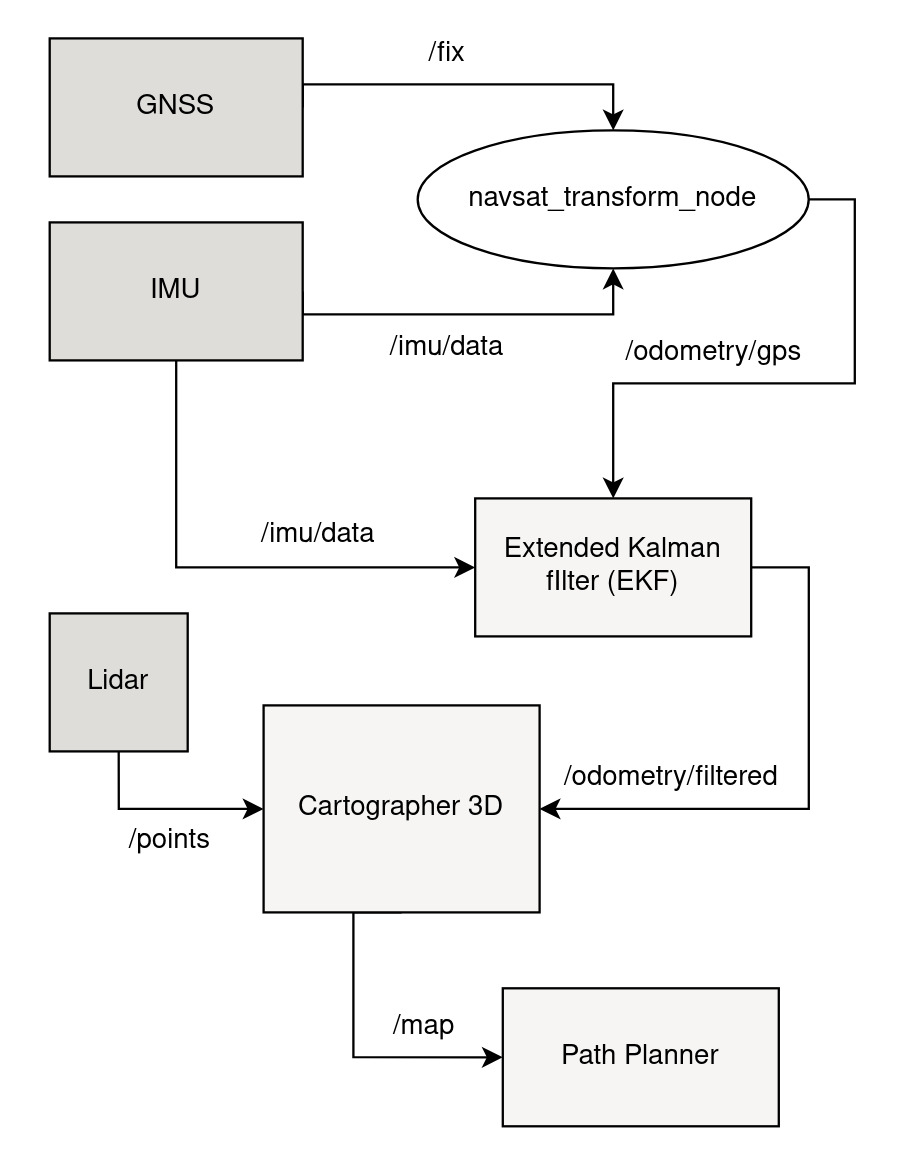
\includegraphics[scale=0.2]{images/SLAM.jpeg}}
\caption{High-level SLAM Architecture}
\label{fig}
\end{figure}

\section{Path Planning}
For path planning, the pure pursuit tracking algorithm \cite{b16} was used to compute steering commands required for the vehicle to follow the desired path in real time. The method works by continuously selecting a goal point on the planned path ahead of the vehicle's current position at some lookahead distance \textbf{L\textsubscript{d}}. The algorithm features a lookahead distance of 2.5-5m that is adaptively adjusted based on the car's current velocity to improve tracking stability based on the path's curvature. The lookahead distance is calculated by:
\begin{equation}
L_d = K_{ld} \times V + L_{fc}
\end{equation}

Where \textbf{‘L\textsubscript{d}'} is the dynamic lookahead distance, \textbf{‘L\textsubscript{ld}'} is the speed gain constant, \textbf{‘V'} is the instantaneous forward velocity of the vehicle, and \textbf{‘L\textsubscript{fc}'} is the minimum lookahead distance. 

Once the goal point is identified, the algorithm determines the required steering angle by using the formula:
\begin{equation}
\delta = \arctan\left(\frac{2L \sin(\alpha)}{L_d}\right)
\end{equation}

Where \textbf{‘L'} is the wheelbase of the vehicle, $\alpha$ is the angular deviation between the vehicle's heading and the vector connecting the real axle to the lookahead point, with \textbf{‘L\textsubscript{d}'} being the lookahead distance.

The calculation is repeated for each control cycle, ensuring the vehicle constantly aligns with the updated path based on the latest cone detections. Unlike map-based navigation systems, this implementation operates in a dynamic and unstructured environment where the vehicle relies solely on visual cone detection to build a local track representation. Hence, Pure Pursuit is preferred for its computational simplicity, low latency, and closed-loop geometric control, making it robust to perception noise and irregular cone spacing. Once the vehicle has run through the track once and mapped out the environment, it can move ahead and build an optimised path using algorithms such as MPC (Model Predictive Control).

\section{Performance Evaluation and Optimisation Plan}

While the autonomous system is fully functional, the team is actively working on the following optimisations to enhance its performance and achieve its full potential. The team has identified areas where the autonomous system falls behind in terms of performance.

\subsection{CUDA for Raw data acquisition}
While a multi-threaded approach using mutually exclusive locks is currently employed for transforming 3d point cloud data into the vehicle’s reference frame, CUDA (Compute Unified Device Architecture) is being incorporated to enhance the system’s real-time performance, scalability, and computational efficiency, particularly as sensor resolution and update rates increase. Benchmarks have demonstrated that GPU-accelerated implementations can outperform multi-core CPU methods by substantial margins\cite{b17}. For instance, a study reported that transforming 100 million vertices took approximately 0.096 seconds using CUDA, compared to 0.508 seconds with a CPU-based approach, indicating a speedup of over 5 times\cite{b18}.

\subsection{MPC}
While a Pure Pursuit algorithm is already implemented for path tracking in the system, MPC (Model Predictive Control) will be incorporated to enhance the controller’s ability to consider dynamic constraints, improve tracking accuracy, and ensure smoother trajectory following under more variable driving conditions.

The advantage of MPC lies in its ability to calculate high-precision control inputs within a limited prediction horizon, based on the vehicle model and reference trajectory. It uses a mathematical representation of the plant to predict the future, and together with a cost function, outputs the optimal control inputs.  The vehicle kinematic or the bicycle model describes the vehicle's motion in terms of position and orientation on the track. Aiming to implement this ‘bicycle model’ to describe the car's dynamics and assume constant normal tire load, i.e., F\textsubscript{zf}, F\textsubscript{zr} = constant, as this model captures the most relevant non-linearities associated with lateral stabilisation of the vehicle. 

The following is the cost function in MPC:

\[
J = \sum_{k=0}^{N} \left[ 
\underbrace{\lambda_y (y_k - y_{\text{ref},k})^2}_{\text{Cross-track error}} + 
\underbrace{\lambda_\psi (\psi_k - \psi_{\text{ref},k})^2}_{\text{Heading error}} + 
\underbrace{\lambda_\delta \delta_k^2}_{\text{Steering effort}} 
\right]
\]

where \textbf{‘J'} represents the total cost, \textbf{‘N'} is the prediction horizon, and \textbf{‘k'} is the current step, ranging from \( 0 \) to \( N-1 \). \textbf{‘$\lambda$\textsubscript{y}'} is the weight for the cross-track error, while \textbf{‘y\textsubscript{k}'} denotes the vehicle's lateral position at step \( k \), and \textbf{‘$y_{\text{ref},k}$’} is the reference lateral position at step \textbf{‘k’}. \textbf{‘$\lambda$\textsubscript{$\psi$}’} represents the weight for the heading error, with \textbf{‘$\psi$\textsubscript{k}’} being the vehicle's heading at step \textbf{‘k’} and \textbf{‘$\psi$\textsubscript{{ref, k}}} the reference heading at step \textbf{‘k’}. Finally, \textbf{‘$\lambda_{\delta}$’} is the weight for the steering effort, and \textbf{‘$\delta$\textsubscript{k}’} is the steering angle at step \textbf{‘k’}.

\bibliographystyle{ieeetr}
\bibliography{references/references}
\vspace{12pt}

\end{document}
